\chapter{Methodology}
%Purpose of Study
The purpose of the research is to evaluate the capability of RTK augmented GPS/GNSS to safely, rapidly, and precisely measure track position employing common track vehicles such as HiRails and locomotives as a survey platform. Figure~\ref{fig:plan} describes the major goals and their relationship in meeting the research objectives. Rail transportation needs were identified from interviews with rail company experts, an assessment of current railroad process and capabilities, observation of yard operations in light of the expert interviews, and the identification of a statewide CORS network accessible to researchers. Additional interviews with subject matter experts has led to the design of experiments that can be performed within the safety and access constraints of a Class I railroad.

Three experiments were designed to examine the use of RTK augmented GPS/GNSS over yard and mainline railway to evaluate the vertical precision, horizontal accuracy, and the reliability of RTK augmentation to measure track position and determine track occupancy.
\begin{enumerate}[1)]
	\item RTK GPS will be used in a automatic classification yard to produce track profiles.
	\item RTK GPS/GNSS will used to produce horizontal track alinement information.
	\item RTK GPS/GNSS will be evaluated for the ability to provide reliable indication of track occupancy.
\end{enumerate}
% Research questions
The research will investigate the use of Real Time Kinematic (RTK) augmentation to the Global Positioning System (GPS) and Global Navigation Satellite Systems (GNSS) with three experiments. The experiments seek to determine if RTK GPS/GNSS augmentation can enable safe and rapid track observations for use in evaluating track infrastructure.

\begin{flushleft}
\emph{Vertical Precision:}
Can a locomotive use RTK augmented GPS to measure the  vertical profile of bowl tracks in an automatic classification yard during production activity?

\emph{Horizontal Accuracy:}
Can a common track vehicle use RTK augmented GPS/GNSS to determine the horizontal degree of curvature comparable with specialized track geometry vehicles?

\emph{Reliability:}
Can a common track vehicle use RTK augmented GPS/GNSS to meet the positioning requirements for track occupancy outlined by the FRA for a location determination system?
 \end{flushleft}
			%%%%%%%%%%%
			% Research Design %
			%%%%%%%%%%%
\section{Research Design and Data Collection}

% Research Plan Diagram
\begin{figure}[!h]
	\centering
	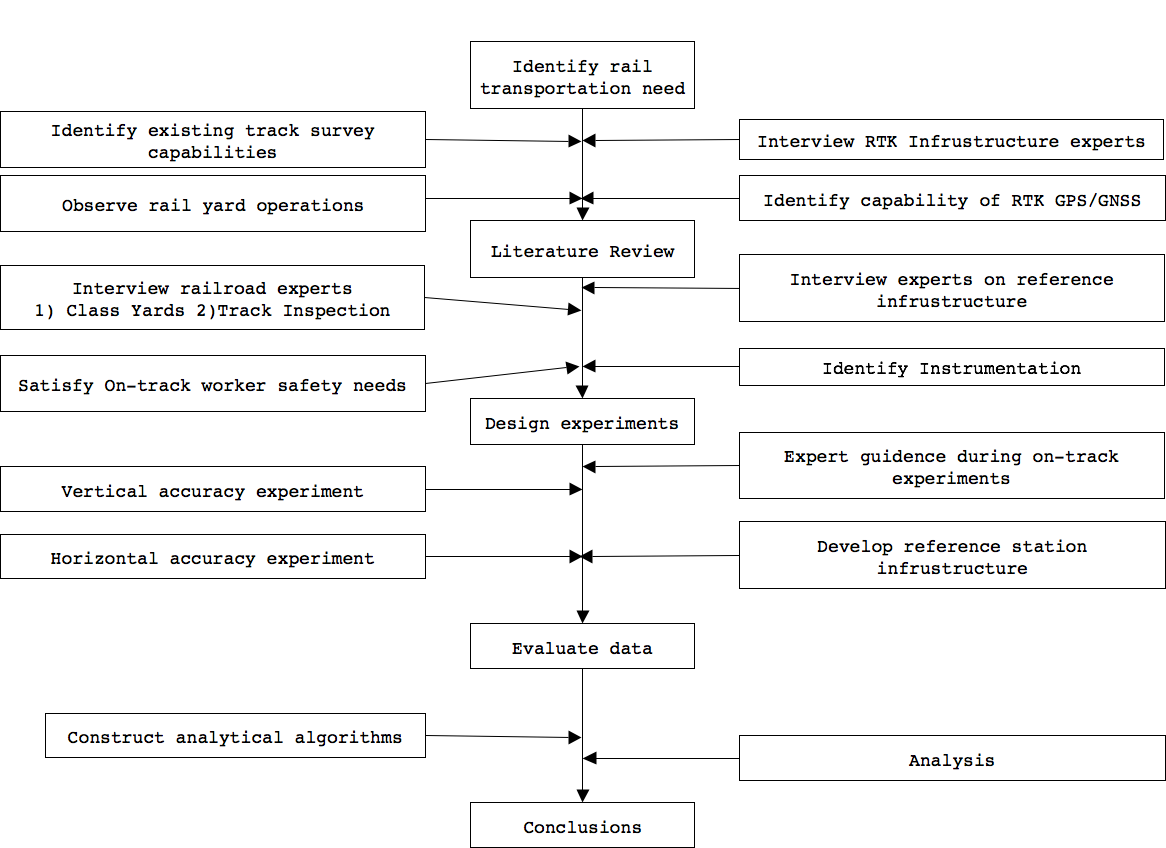
\includegraphics[width=6in]{research_plan.png}
	\caption{Research Plan}
	\label{fig:plan}
\end{figure}
The research will investigate the capability of RTK GPS/GNSS augmentation over active track. Federal and private property laws restricts access to active track. Therefore all research activities will be performed in accordance with 49 CFR \S214 railroad workplace safety regulations, subpart C \textit{Roadway Worker Protection}~\citep{49CFR214300} and subpart D \textit{On Track Roadway Maintenance Machines and HiRail Vehicles}~\citep{49CFR214500} as well as rail company rules and procedures specific the the research location. 

An evaluation of RTK augmented vertical measurement will be made by single epoch observations of track position by locomotive across an active hump yard. The track positions will be used to produce profiles for each bowl track.

An evaluation of RTK augmented horizontal performance will be made using single epoch observations of track position by a common track vehicle over active mainline track. Horizontal track alinement will be evaluated by determining the degree of curvature from track observation.

An evaluation of RTK augmented position reliability will be made by a common track vehicle over active mainline track. Multiple track positions over identical segments will evaluated against previously produced track geometry. Track positions will be evaluated for RTK's likelihood of determining track occupancy.

A scope of work with the anticipated timeline for completion of the plan objectives is referenced in figure~\ref{fig:timeline}.

Horizontal coordinates will reference the World Geodetic System 1984 (WGS84) ellipsoid. Vertical coordinates will reference the North American Vertical Datum of 1988(NAVD88). An East, North, Up (ENU) Cartesian coordinate projection will be used for deriving track alinement and position, with coordinate and distance units reported in decimal feet.

The electrical point of reference for a GPS/GNSS antenna is the phase center. The phase center is offset some distance from a physical reference location on the antenna housing. The physical antenna reference for each of these experiments will be the antenna mounting point. The survey controller will contain a table of offset distances between phase center and mounting point for the antennas used during each experiment. A procedure to align the antenna mounting point on the track vehicle with a track reference location (i.e.\ centerline, left or right rail) will be performed as part of the mobile track vehicle setup.

Estimates for the horizontal and vertical precision are calculated by the GPS/GNSS receiver. This estimate is the product of the geometric dilution of precision (GDOP) and the user-equivalent range error (UERE). The GDOP is determined by the geometry of the SV constellation in view, while the UERE is considered the statistical sum of the contribution from each of the error sources associated with a visible space vehicle~\citep{2004leick,Kaplan}.

The observation procedure for these experiments progress from setup of the reference station or reference network; establishing a means of communication between the reference station/network and the track vehicle; aligning the antenna and configuring the mobile receiver onboard the track vehicle.

%Hump yard profile design
\subsection{Experiment One: Vertical Precision} \label{ResDHmpYd}

Can a locomotive use RTK augmented GPS to measure the  vertical profile of bowl tracks in an automatic classification yard without the need for track closures?

The objective of experiment one is to use a locomotive to survey an active hump yard to produce track profiles from RTK augmented track observations.
%{Ad Hoc Base Station Procedure}
The hump yard survey will use a single RTK reference station transmitting correctors via UHF radio to a mobile receiver onboard a locomotive.  The reference station components for this experiment will consist of a reference station receiver, reference station antenna, and a UHF data radio. A fixed-height tripod to support the GPS and UHF antennas will be set up on the highest point available at the yard to provide minimal obstructing SV signals and maximize height above average terrain (HAAT) for UHF data reception by the roving receiver. The reference station will record observations during several four to eight hour sessions. The compressed observations will be converted to the Receiver INdependent EXchange (RINEX) format and processed through the National Geodetic Survey Online Position User Service (NGS OPUS) to adjust the position of the reference station position.

RTK correctors broadcast from the reference station by UHF data radio will augment the GPS receiver position aboard the locomotive. A survey controller connected to the receiver will manage automated data collection and record single epoch observations with a nominal horizontal separation of ten feet. Track profiles will originate at a common reference point at the hump end terminating at the pullout-end switch for a particular track.

Points of interest such as switches, wheel detectors, and retarder inlet and outlets locations will be surveyed using the static survey instrument on the ground using watchman-lookout protection during the brief period.

Aggregate track observations will be deconstructed to individual track segments and be assigned a linear reference location. 

Experiment one will:
\begin{enumerate}
	\item  Collect continuous single epoch observations on a nominal 10 foot horizontal spacing with RTK augmented GPS onboard a locomotive in an active hump yard. 
	\item Produce a plan view color mapped elevation drawing for the bowl area of the yard.
	\item Produce a plan view color mapped vertical precision drawing for the bowl area of the yard.
	\item Produce two-dimensional profile drawings for each track.
	\item Determine the descriptive statistics for the performance of RTK augmented GPS vertical elevation as measured by a locomotive.
\end{enumerate}
\emph{Variables of analysis}: A three dimensional (ENU) coordinate will consist of:
\begin{itemize}
\firmlist	
	\item Northing
	\item Easting
	\item Elevation
	\item Vertical precision estimate
	\item Time and date of observation
	\item A count of the SVs in view of the mobile receiver
	\item Vertical Dilution of Precision (VDOP), a measurement of the geometry of the SVs in view
\end{itemize}
% Mainline Track alinement design
\subsection{Experiment Two: Horizontal Accuracy}
\label{Ex2Design}
Can a common track vehicle use RTK augmented GPS/GNSS to determine the horizontal degree of curvature comparable with specialized track geometry vehicles?
The objective of experiment two is to perform a mainline track survey to produce horizontal track alinement from RTK augmented track observations. The track alinement survey will use a network of CORS RTK reference stations located along the survey route to stream observations to a central Virtual Reference Station (VRS) server. A public cellular data service will transmit correctors from the VRS to a mobile receiver onboard a track vehicle. A survey controller connected to the mobile receiver will record single epoch observations with a nominal horizontal separation of ten feet. 
% FRA alinement figure
\begin{figure}[!htp]
	\vspace{-30pt}
		\begin{center}
			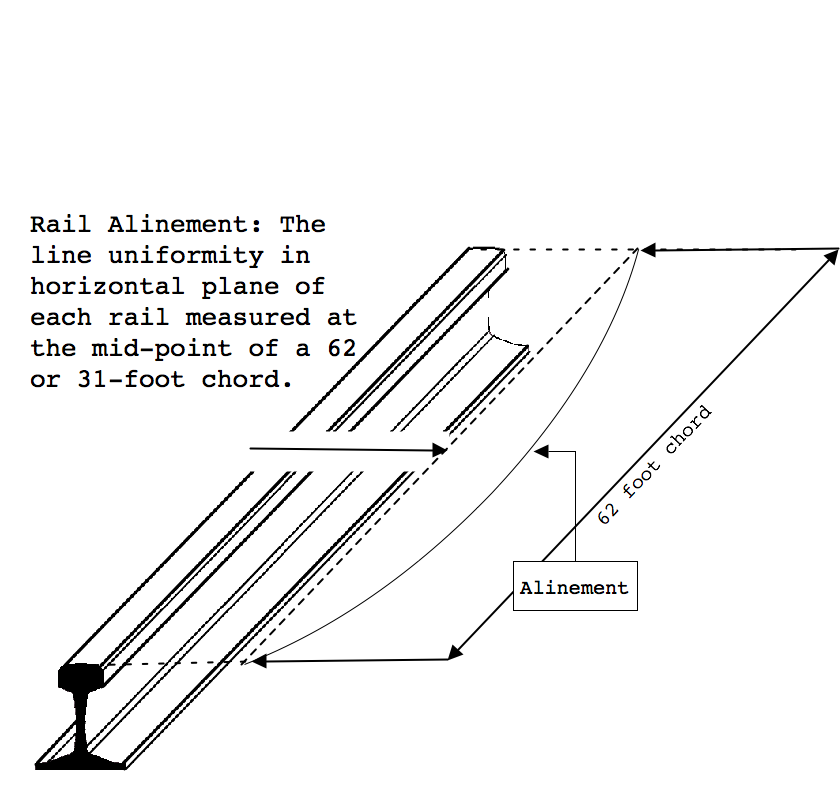
\includegraphics[width=3in]{HorzAlignment.png}
			\caption{Horizontal Alinement}\label{fig:Alinement}
		\end{center}
	\vspace{-30pt}
\end{figure}

The track observation data will be used to find the degree of curvature using a software modeling the standard string lining method  for railways.
Experiment two will:
\begin{enumerate}
	\item Collect continuous single epoch observations on a nominal 10 foot horizontal spacing with RTK augmented GPS/GNSS on board a track vehicle over at least 30 miles of mainline track.
	\item Develop a software model for calculating the radius of curvature from RTK augmented GPS/GNSS track vehicle observations. The software will model the string lining method described in the FRA \emph{Track Safety Standards Compliance Manual}~\citep[pp.26-30]{2007FRATrack} using a 62 foot chord length on 15.5 foot stations.
	\item Graphically correlate RTK augmented GPS/GNSS alinement determined from the software model plotted with track geometry car degree of curvature over identical track sections.
	\item Determine the horizontal alinement variability of the horizontal alinement found from RTK augmented GPS/GNSS observations in select tangent segments.
\end{enumerate}

\emph{Variables of Analysis}: Three dimensional (ENU) coordinates will consist of:
\begin{itemize}
	\item Northing
	\item Easting
	\item Elevation
\end{itemize}
% Track Occupancy Design
\subsection{Experiment Three: Reliability} 
Can a common track vehicle use RTK augmented GPS/GNSS to meet the positioning requirements for track occupancy outlined by the FRA for a location determination system?

The objective of experiment three is to determine how reliably RTK augmentation can reproduce the position of track vehicle as an aid to determining track occupancy. The track occupancy experiment will use a network of CORS streaming observations to a central server farm. A mobile receiver onboard a track vehicle will use a public cellular data service to securely access correctors transmitted to the receiver by the VRS. A survey controller connected to the receiver will record single epoch observations with a nominal horizontal separation of ten feet.

Multiple sets of mainline track observations will be used to find a mean location of tangent and circular track geometries by least-squares linear regression. The distance between individual observations from a each traverse of the track geometry determined by regression will be used to determine if RTK augmented GPS/GNSS can reproduce track position with sufficient statistical significance to meet the FRA requirement for a location determination system.

Experiment three will:
\begin{enumerate}
\item  Collect continuous single epoch observations on a nominal 10 foot horizontal spacing with RTK augmented GPS on board a track vehicle over at least 30 miles of mainline track.
\item Determine an average track position for selected tangent and circular curve segments from continuous track vehicle observations.
\item Determine the distance from subsequent observations by track vehicle to the reference tangent and curve geometry.
\item Determine if statistical evidence exists to indicate if RTK augmentation of GPS/GNSS is capable of determining the track occupancy of a vehicle meeting FRA performance standards of a location determination system.
\end{enumerate}
\emph{Variables of Analysis}: Three dimensional (ENU) coordinates will consist of:
\begin{itemize}
	\item Northing
	\item Easting
	\item Elevation
\end{itemize}
			%%%%%%%%%%
		        % Instrumentation %
			%%%%%%%%%%
\section{Instrumentation}\label{instrumentation}
Instruments to be used in the research are summarized in table \ref{tab:instruments}.
% Table of instrumentation
\begin{table}[ht]
	\begin{center}
	\caption{GPS/GNSS Instrumentation}\label{tab:instruments}
	\begin{tabular}{llll}%{ p{2.0cm} p{3cm} p{3cm} p{3cm}}
	\toprule
	Unit & Instrument & Description &  Experiment\\
	\midrule
	Ad hoc& Trimble 5700 & 24 ch. GPS rcvr & 1\\
	Reference& Zephyr Geodetic & GPS antenna w/GP & \\
	Station& Trimmark III UHF radio & 450Mhz band& \\
	\midrule
	CORS & NetRS/NetR5 & 24/72 ch. GPS &\\
	& Trimble Zephyr Geodetic & GPS/\-GNSS antennas & 2, 3\\
	\midrule
	VRS & Trimble Network Infrastructure & Server software & 2, 3\\
	\midrule
	Static Module & Trimble R8 & 24 ch. GPS w/int. radio &1\\
	& Trimble TSC2 & Survey Controller &\\
	\midrule
	Mobile\#1 & Trimble 5700 & 24 ch. GPS w/int. radio & 1\\
	& Trimble TSC2 & Survey Controller &\\
	Mobile\#2 & Trimble R7 & 72-ch. GNSS receiver& 2, 3\\
	& Trimble TSC2 & Survey Controller &\\
	\bottomrule
	\end{tabular}
	\end{center}
\end{table}
\begin{itemize}
	\item An ad hoc reference station (AhRS) as listed in table \ref{tab:instruments} uses a stationary reference antenna to receive SV signals for manipulation by a GPS receiver to produce correctors for transmission over UHF data radio to a capable mobile GPS receiver.
	\item A continuously operating reference station (CORS) provides continuous data for RTK surveying applications.
	\item Virtual Reference System (VRS) is a network of CORS that enable RTK augmented GPS/GNSS positioning over a wide area, eliminating the need to position ad hoc reference stations along the survey route. A VRS network is made up of GPS/GNSS CORS hardware, modeling and networking software, plus a communications interface. RTK mobile receivers are able to securely access a VRS real-time network modeled correction with system integrity monitoring that warns of any data problems.
	\item A static survey unit is an RTK enabled GPS/GNSS receiver used by a surveyor to determine the coordinate of a position by recording an average of multiple-epoch observations while occupying the point of interest.
	\item A mobile survey unit is an RTK enabled GPS/GNSS receiver used to determine the coordinates of a position while in motion by recording single epoch observations.
\end{itemize}
			%%%%%%%%%%%%%%%%
			%  Data Validity and Integrity %
			%%%%%%%%%%%%%%%%
\section{Data Validity and Integrity}
The number of observations generated during each experiment can estimated by simply dividing the length of track to be surveyed in feet by the nominal distance between observations. Table~\ref{tab:dataEst} provides an estimate for the number of observations expected from each experiment.

% Table of instrumentation
\begin{table}[ht!]
	\begin{center}
	\caption{Data Estimate by Experiment}\label{tab:dataEst}
		\begin{tabular}{c c c}
		\toprule
		Experiment & Est. Length & Est. Observations\\
		\midrule
		1 & Hump yard, 58 tracks x 2,000 ft & 11,6000 \\
		2 & Single mainline traverse of 30 miles & 15,800\\
		3 & Three mainline traverses of 30 miles & 47,400\\
		\bottomrule
		\end{tabular}
		\vspace{-20pt}
	\end{center}
\end{table}
% Validity
\emph{Validity}

Insuring the the validity of these data will rely on the quality control performed by the data collector software. A field notebook will be kept to record values (i.e., antenna height from top of rail, locomotive number, track reference point) found during antenna alinement. The recorded values will be programmed in the controller as a specific survey style to insure using identical calibration values between observation files during multi-day surveys. The TSC2 survey controller will be programmed to reject observations that fall outside threshold values for horizontal and vertical precision. Threshold values will be selected that balance the continuous recording of all data with observation precision. In this way the survey controller software will act as a filter to eliminate outliers.

Plotting experiment one observations using ESRI ArcMap software allows a three-dimensional examination for groups that have consistent higher or lower elevations than other observations. This information will be examined for indications that a blunder may have occurred as the result of incorrectly entered antenna elevation offset.

Experiment two observations will be checked to insure the observations are continuous by using the software to flag a change in bearing between any two observations that approaches 180$^{\circ}$, indicating the track vehicle backed up while recording observations. Observations generated by inadvertent recording in this manner will be deleted.

% Integrity
\emph{Integrity}

The elevation integrity of observations will be maintained by using NAVD83 and avoiding `mixing' datums within or between experiments~\citep{NGSBluebookX1}. 

During experiment one, several hundred points of interest (i.e., track switch points, retarder inlet and outlet, wheel detectors) will be surveyed on the ground. This data will be adjusted such that the POI is perpendicular to the rail and coincident with the track reference point.  Maintaining the integrity of the adjusted observations will be performed graphically by plotting the adjusted points with the track vehicle observations to verify the adjusted POI is properly located.

Management of some data will use a web-based spreadsheet to provide collaboration between researchers. Data integrity will be enhanced due to the `change logging' and `previous version rollback' features of the web-based spreadsheet.

				%%%%%%%%%%
				%  Data Analysis %
				%%%%%%%%%%
\section{Data Analysis}

The analytical objectives referenced in figure \ref{fig:plan} will combine quantitative measurement with a qualitative evaluation of track observations produced by mobile track vehicle equipped with RTK augmented GPS/GNSS instrumentation. Observations are collected by a survey controller and are transferred to \emph{Trimble Geomatic Office} (TGO) software where any reference station location adjustments will be propagated to each observation.

The adjusted observations will be exported from the TGO software in a format that includes each observation name (coded by track segment), feature code (i.e., centerline, switch point, wheel detector, retarder inlet), northing, easting, elevation, horizontal and vertical precision, time and date, and number of SVs. The variables of analysis used in a particular experiment will be extracted from the export file.

Mainline track locations are reported as a linear reference from a wayside mile post monument. A track reference uses the mile post number plus the offset from the monument in decimal miles. Mile post references are typically measured by odometer, therefore the offset distance from the mile post is the accumulated slope distance. In addition, the slope distances between mile posts over railways in the United States is not a constant measure. To determine a mile post reference location, the number of feet offset from a mile post monument to the desired location is divided by distance between mile posts in feet plus the mile post number\footnote{Assumes increasing mile post numbers, subtract if decreasing.}.

% Experiment 1 Analysis
\subsection{Experiment 1: Vertical Precision}

Hump yard track observations collected from onboard a locomotive will be exported from the survey controller to TGO. Observation coordinates will be adjusted by using the ad hoc reference station location determined from observing sessions processed by the National Geodetic Survey (NGS) \emph{Online Position User Service} (OPUS). Observation sessions will be a minimum of four hours in length.

The OPUS-derived position will be substituted for the reference station initial autonomous position, with the track observations recalculated from the observation vectors by TGO. The reference station observations will be concatenated and converted to the Receiver INdependent EXchange (RINEX) format. The resulting observation and and navigation files will be processed using UNAVCO TECQ (translation, editing, quality check) software. The TEQC report will be examined for anomalous site or receiver influences, such loss of L1 and/or L2 signal, ionospheric and multi-path phase slip, receiver clock slip, and blocked SV signals in relation to poor vertical precision observations.

Further adjustment to track elevations will made by observing any survey monuments found proximal to the yard. Monuments will observed for at least 180 epochs. The current NGS Permanent Identification (PID) datasheet value will used to adjust the AhRS elevation.

The yard observations will be separated into layers organized by lead, group, and track. Deconstructing the aggregate observations enables individual tracks to be configured from a continuous series of points from the hump lead through the main, intermediate and group retarders, group, lead, and bowl tracks by activating the correct layers in TGO. A properly configured track will be apparent as a continuous series of points extending from the hump to the pullout end.

Locations of track points of interest (i.e., track switch points, retarder inlet and outlet, wheel detectors) are associated with a position nearest a particular rail. The POI will be observed at the center top-of-rail nearest the POI physical location using the static survey instrument. The position of the points of interest will be adjusted in the office to be perpendicular with the center top-of-rail observation and coincident with the track centerline.

Continuous track observation names will be renumbered in series from hump to pull out. Feature coded definitions will enable separation by point type and automatic line work created for the centerline points. The line work and observation data will be exported from TGO in the ESRI\footnote{Environmental Systems Research Institute, Inc.} shapefile format. The point data will also be exported exported as a comma delimited (CSV) file.

The CSV file will be imported to a spreadsheet program, where a linear reference will be found for each point. The elevation and linear reference coordinate will be scaled in the spreadsheet and added to a CAD drawing containing the track design grade\footnote{Provided by the rail company sponsor.}. 

Each track profile will be plotted as an overlay to the provided CAD drawing. The design profile in the CAD drawing is relevant to the rail company in a making a volumetric assessment of surfacing material required to bring the relief of each track into vertical alignment with the design grade. Calculation of surfacing material quantity is outside the scope of the experiment. The design grade and locomotive survey result will be used as a comparative tool, limited to providing track profile deviation from design grade.

The shapefiles will be added to ESRI ArcMap software where a plan view of of the bowl area track elevation and vertical precision estimate will be represented in plan view. The vertical precision map will show lower quality vertical precision for points > 0.1 feet in a contrasting color to those of greater precision. The plot will be examined for the distribution of lower quality data patterns.

Acceptable elevation quality will be apparent as a smooth track profile. Poor quality observations will appear with greater variation between points, resulting in a jagged or sawtooth profile. Poor quality elevations will be identified and correlated with: observation time; vertical precision estimated by the receiver; and reference station observations during the period.

The vertical precision calculated by the receiver will be used to determine descriptive statistics and to plot a histogram for the yard profile survey.

%An analysis of the vertical precision of the observations will be used to determine if statistical evidence is present to indicate the one sigma mean vertical precision of RTK augmented GPS observations by locomotive in a hump yard is 0.1 feet or less.

% Experiment 2 analysis
\subsection{Experiment 2: Horizontal Accuracy}\label{trackAnalysis}

Mainline track observations collected onboard a track vehicle will be exported from the survey controller into \emph{Trimble Geomatic Office} software, examined for blunders, and exported as described previously. Analysis of variables will be processed to determine the degree of curvature, following the string lining method described in Federal Railroad Administration \emph{Track Safety Standards Compliance Manual for track classes 1-5} per 49CFR\S213.55. This method follows the historical use of string lining for determining the degree of curvature on railways~\citep{1964hickerson}.

The software model will use RTK augmented GPS/GNSS ENU observations to find the degree of curvature at points linearly referenced to wayside monuments. The model will determine the coordinates of stations spaced at 15.5 foot intervals.  For each station, a 62 foot chord intersecting a line segment defined by sequential RTK observations will be used to determine the middle ordinate offset for that chord.

Equivalent linear mile post references will be determined from sequential RTK observations by accumulating the slope distance between observations. Since the distance between mile post reference monuments over a railway in the United States varies, it will be necessary to evaluate each mile length independently. A mile post reference location will be determined by adding the mile reference number to the the ratio of the accumulated distance offset from a mile marker and the total distance accumulated between mile markers.

The string lining method as practiced by track inspectors and superintendents determines points of greatest alinement deviation by moving a 62 foot string along the track in increments until the point with maximum deviation is found. The software model will use a similar approach in moving the chord in 15.5 foot stations along lines defined by a series of RTK track observations. The distance from the chord middle ordinate to a line segment defined from RTK track observations will produce the mid-chord offset (MCO).  The software model will determine MCO from RTK augmented GPS/GNSS as represented in figure~\ref{fig:strLining}.

Coordinates for the chord end point are determined by extending a 62 foot radius circle originating from the station coordinates, figure~\ref{fig:strLining} station~($x_o, y_o$). The `chord circle' intersection with a line segment defined from the farthest point inside the chord circle and the nearest point outside the circle determines the chord terminal coordinate. The intersection is indicated at point ($x_{int}, y_{int}$) in figure~\ref{fig:strLining}, lying between points D and E.
	% String Lining Illustration
\begin{figure}[!htp]
	\begin{center}
		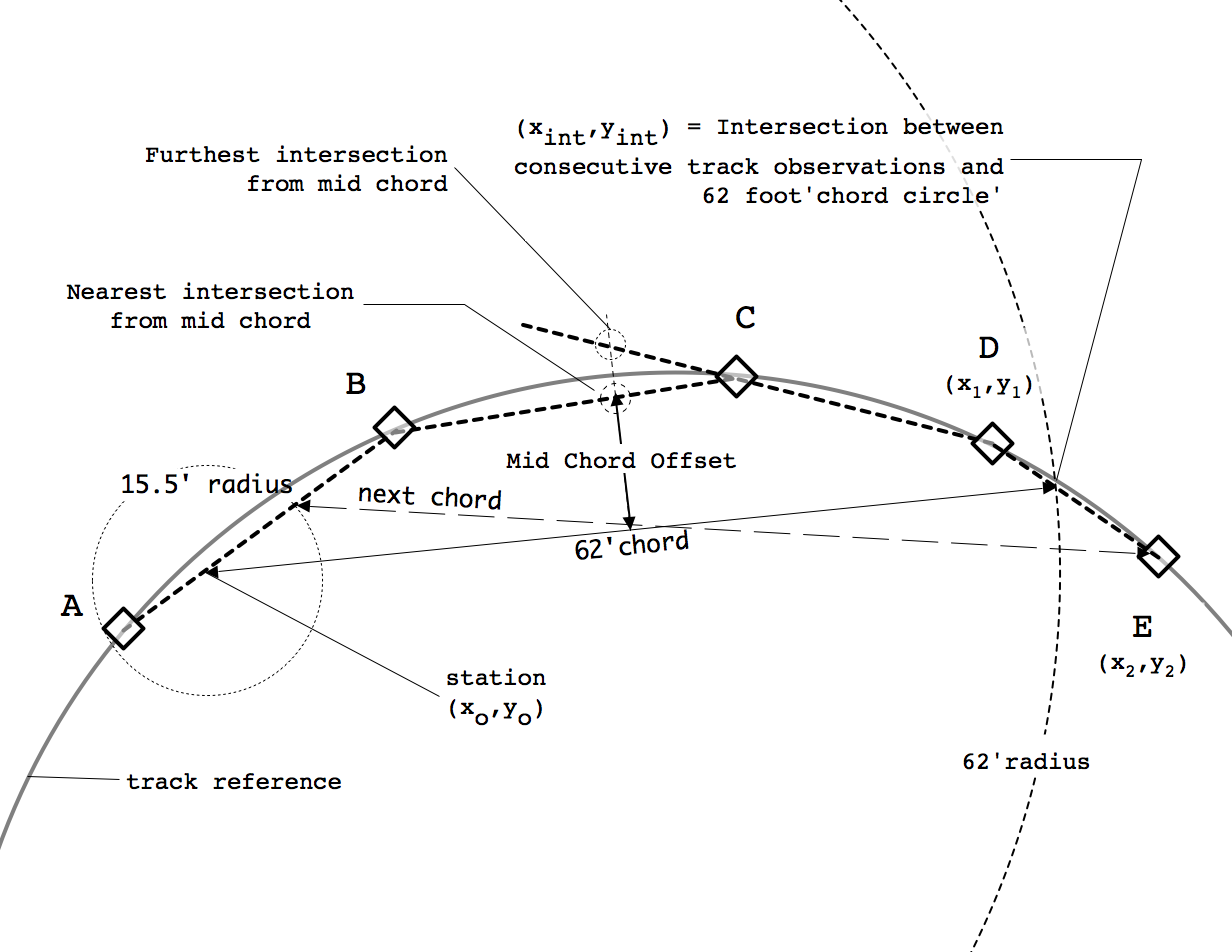
\includegraphics[width=13cm]{stringLining.png}
		\caption{Modeling the String Lining Method from RTK Track Observations}
		\label{fig:strLining}
	\end{center}
\end{figure}
The MCO is determined from an line orthogonal with the chord at the middle coordinate. The the mean distance between the nearest and farthest of two line intersections projected from the three RTK observations nearest the middle ordinate (figure~\ref{fig:strLining} points B, C, and D) and the middle ordinate orthogonal to the chord determines the MCO. The degree of curvature (chord definition) is found from the MCO and chord length in feet by the relationship~\citep{1964hickerson}.
	\begin{equation}
		D_c = \frac{45840 \times MCO}{chord^2}
	\end{equation}
The model will assign a mile post reference to the degree of curvature. The coordinates of the next station will be found by intersecting a 15.5 foot radius curve originating at the current station with a line between observations similar to the procedure for determining the chord terminal coordinates as indicated in figure~\ref{fig:strLining}. 

A railway can be described as a smooth, continuous shape. Therefore, as an aid to exploring track alinement, a smoothing algorithm will be applied to the degree of curvature verses mile post information to filter and reduce the effect of outliers. A local regression smoothing method using a weighted linear least-squares regression will be employed. The optimal span of neighboring data points that produces a smoothed data set that most closely resembles the degree of curvature data from a specialized track geometry vehicle will be found through trial and error.

RTK derived track alinements from different traverses recorded over a time period will be plotted and evaluated for:
\begin{itemize}
	\item Horizontal alinement correlation between track geometry vehicle degree of curvature vs. mile post reference and the degree of curvature found from RTK augmented GPS/GNSS track observations.
	\item Correlate between the horizontal alinement of RTK augmented GPS and augmented GNSS transits across the same track segment.
	\item Determine and compare the degree of curvature variability in select tangent track segments for RTK augmented GPS/GNSS instrumentation and a rail company provided track geometry vehicle data.
\end{itemize}

Tangent segments will be selected from the beginning, middle, and end of the study area. The degree of curvature variance will be determined from selected tangent in those tangent segments. A threshold of $\pm$one-half degree of curvature will be used to determine if statistical evidence is present to indicate comparable performance with a track geometry vehicle.
% track occupancy data analysis
\subsection{Experiment 3: Reliability}

The reliability of RTK augmented GNSS observations to reproduce track position will be determined from track observations during an initial traverse of mainline track with a track vehicle and subsequent traverses. Track observations from sample tangent and circular curve segments will define the tangent and circular geometries by the method of linear least-squares regression. The geometric coefficients defining the tangent and circular track location and the limit of the tangent and curve coordinates will be used as the track reference location.

An objective for a linear regression model is to determine the equation coefficients for tangent and and circular curve geometries through `center of mass' of the track observations.

In the case of tangent segments, RTK track vehicle coordinates will be treated as a point on a line parallel with the tangent segment. The distance between the reference tangent and observed point will be determined by finding the distance between the two parallel lines.

In the case of circular segments, subsequent observation coordinates will be treated as a point on a circle parallel to the reference circular segment and sharing the same origin. The distance between the reference curve and the observed point will be determined by finding the difference between the curve radius and vehicle coordinate distance from the curve origin.

The mean distances between traverses over for selected geometry segments will be evaluated for conformity with the FRA specification for a LDS used in PTC. 

% Summary
% Summarygoes back to problem statement
\section{Summary}
The research will explore the use of RTK augmented GPS/GNSS in dynamic track measurement experiments. Each experiment will examine the value of RTK augmentation to provide track measurements in the vertical and horizontal plane and well as examining the reliability of single epoch RTK enabled observations to act as a component of a location determination system.

Experiment 1 will evaluate the vertical precision of RTK augmented GPS by setting up a locomotive with mobile survey-grade GPS instrumentation to record a track position every ten feet across an active automatic classification yard. The recorded positions will be used to produce a profile for each track. The mean vertical precision for the bowl area of the yard will be determined from the mobile receiver's precision estimate. A threshold of 0.1 feet will be used as a gage of acceptable RTK vertical precision in this experiment.

Experiment 2 will evaluate the horizontal accuracy of RTK augmented GPS/GNSS performance by setting up a mobile track vehicle to record track position every ten feet on active mainline track across a wide area. Horizontal track alinement will be evaluated by finding the degree of curvature from track observations. The degree of curvature variation across selected tangent track segments will be found and compared with the variation of a specialized track geometry vehicle. A mean variation of $\pm$~one-half degree of curvature will be used as a threshold to gage acceptable RTK horizontal accuracy in this experiment. 

Experiment 3 will evaluate RTK augmented GPS/GNSS position reliability by observing track position by a common track vehicle over active mainline track, and using the track coordinates to determine coefficients for straight and circular geometries over selected track segments. A subsequent traverse recording RTK positions will be evaluated against the straight and circular geometries to determine the mean distance between traverses. The distances will be used to provide an estimate of the likelihood of determining track occupancy using RTK augmented GPS/GNSS meeting FRA guidelines for a location determination system in positive train control applications.

The research timeline represented in figure \ref{fig:timeline} was developed from the research plan in figure \ref{fig:plan}.
\begin{landscape}
	\begin{figure}[htbp]
		\begin{center}
			\vspace{50pt}
				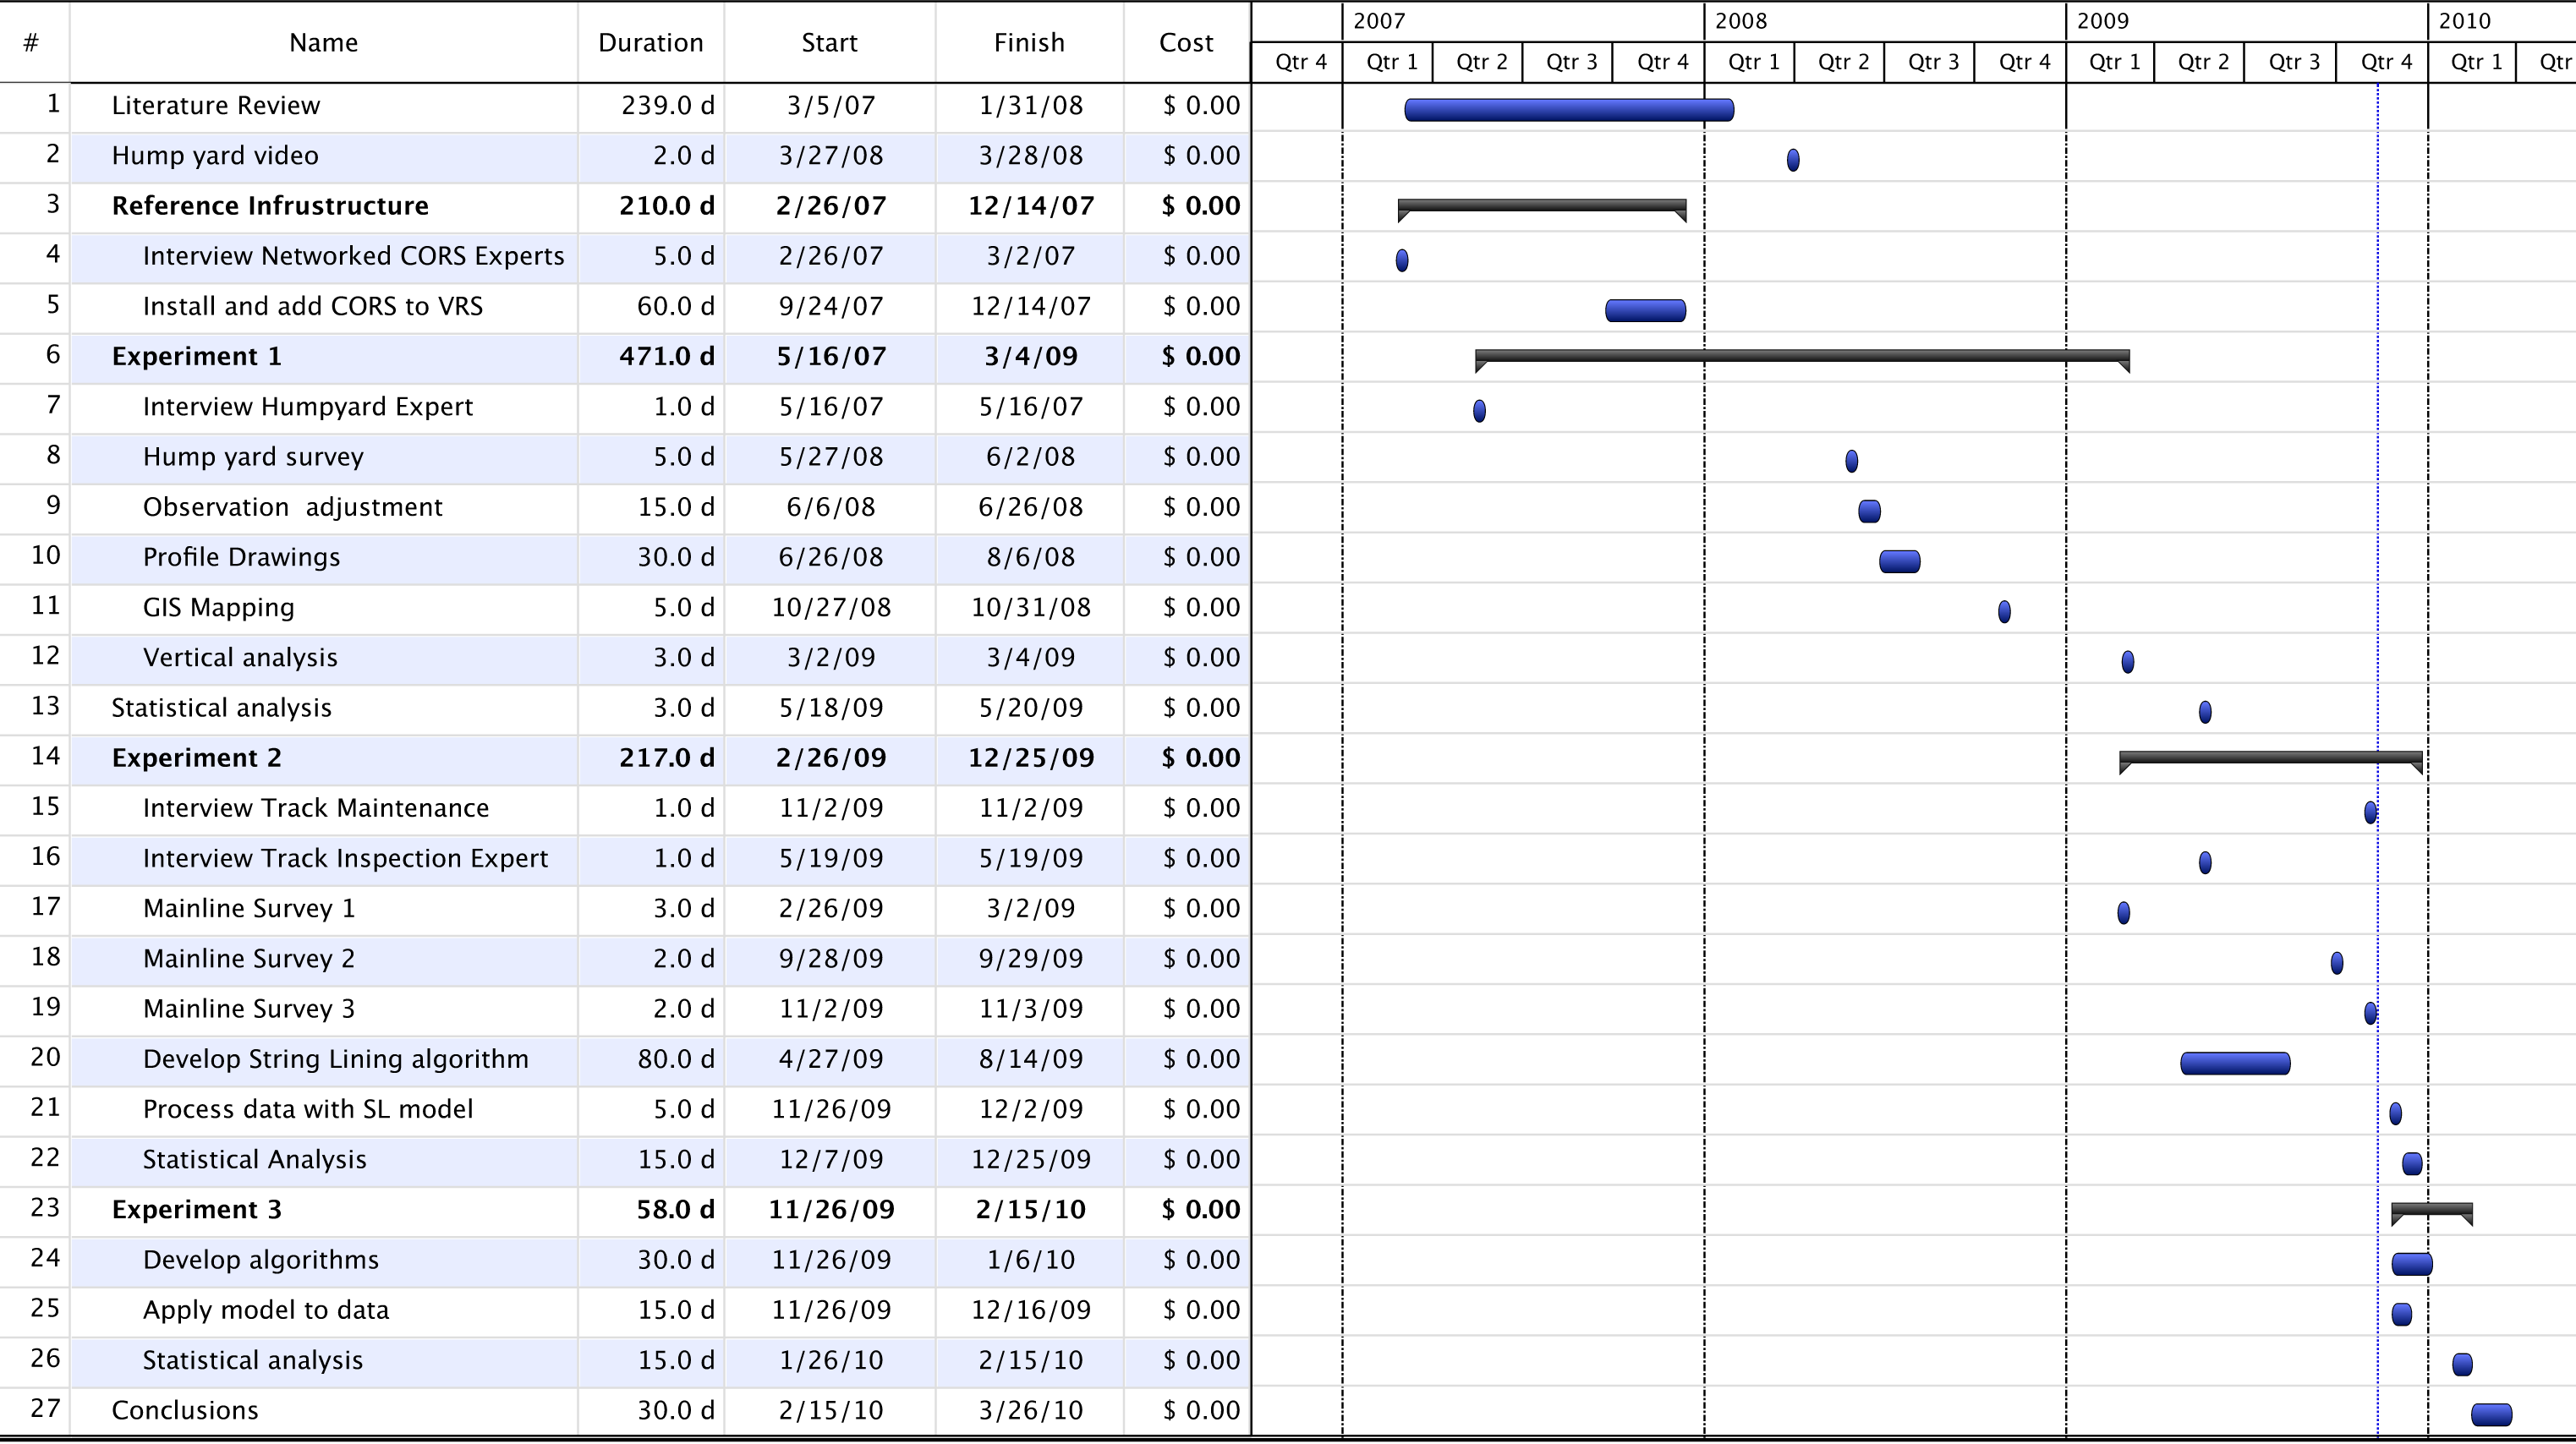
\includegraphics[width=20cm]{ResearchTimeline.png}
			\vspace{30pt}
		\caption{Research Timeline}
		\label{fig:timeline}
		\end{center}
	\end{figure}
\end{landscape}
